%
%%%%%%%%%%%%%%%%%%%%%%%%%%%%%%%%%%%%%%%%%%%%%%%%%%%%%%%%%%%%%%%%%%%%%%%%%%%%%%%
% The LHC
%%%%%%%%%%%%%%%%%%%%%%%%%%%%%%%%%%%%%%%%%%%%%%%%%%%%%%%%%%%%%%%%%%%%%%%%%%%%%%%
%
\chapter{The ATLAS Detector at the LHC}\label{ch:lhc_atlas}

\section{The Large Hadron Collider}


The Large Hadron Collider  (LHC)~\cite{Breskin:1244506} is a proton-proton ($pp$) synchrotron located in the previous Large Electron Positron (LEP) collider tunnel at CERN Laboratory, just outside the city of Geneva (Switzerland), approximately 100~m underground. It is designed to collide bunches of up to $\sim 10^{11}$ protons every 25~ns at a center-of-mass energy of 14~TeV (seven times the 2~TeV reached by the Tevatron accelerator at Fermilab Laboratory, in Chicago). 

The experiments analyzing the collisions produced by the LHC are distributed around the 27~km ring at the various interaction points. The ATLAS experiment is located at Point 1, which is closest to the main CERN site. Point 5 houses the other general purpose detector, CMS. ALICE and LHCb experiments are located at Point 2 and Point 8, respectively. The former is designed to investigate heavy ion collisions; the latter, to investigate rare decays of $b$-mesons. The layout of these four experiments along the LHC ring is shown in Fig.~\ref{fig:LHC1}.

\begin{figure}[htbp]
  \begin{center}
      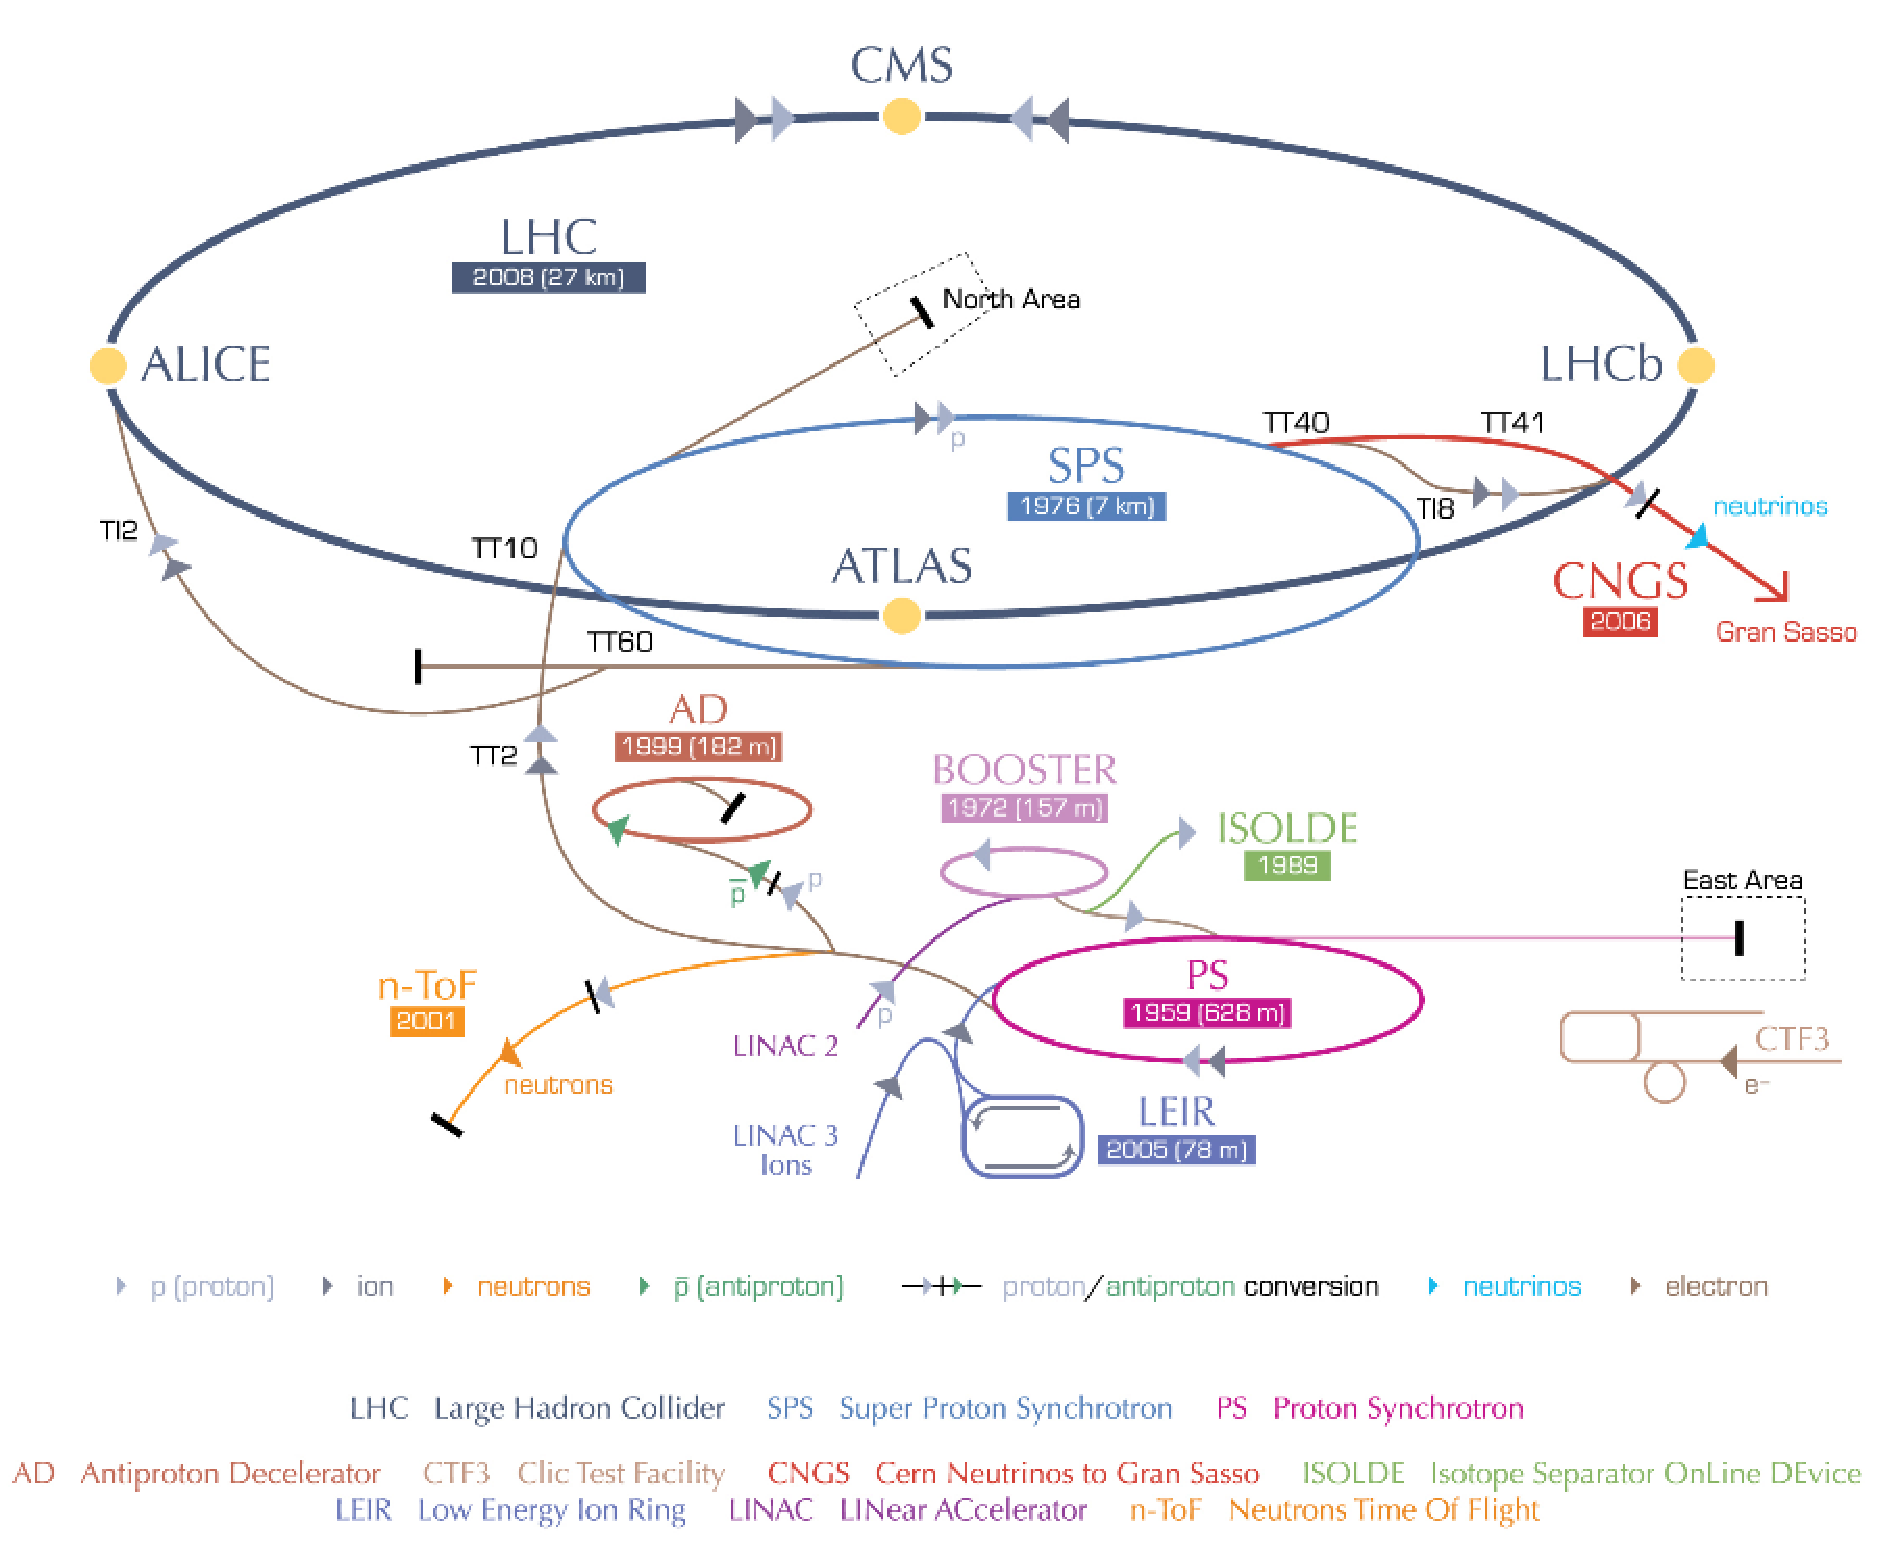
\includegraphics[width=1\textwidth]{Fig2/CERNacceleratorcomplexCut.pdf}
    \caption{The CERN accelerator complex, showing the injection system, along with each component's date of construction, and the placement of the four main experiments.}
    \label{fig:LHC1}
  \end{center}
\end{figure}


Proton beams are formed, before insertion into the main LHC ring, using a succession of smaller machines with increasingly  higher energies, as shown in Fig.~\ref{fig:LHC1}. The chain begins as protons are injected into the PS Booster (PSB) at an energy of 50~MeV from Linac2. The booster accelerates them to 1.4~GeV. The beam is then fed to the Proton Synchroton (PS) where it is accelerated to 25~GeV. At desin strength, the bunch structure, known as a bunch train, contains 72 bunches of protons upon entry to the Super Proton Synchrotron (SPS). The SPS accumulates up to four fills of 72 bunches from the PS and accelerates them to 450~GeV, with a bunch spacing of $\sim$~25~ns. They are finally transferred to the LHC (both in a clockwise and an anticlockwise direction) where they are accelerated for 20 minutes to their nominal energy of 7 TeV. Beams will circulate for many hours inside the LHC beam pipes under normal operating conditions.

The bunch structure is a direct consequence of a radio frequency (RF) acceleration scheme used to attain the desired high proton beam energy.  In RF acceleration, particles travel through a series of time-varying electrical fields and they can only be accelerated when the RF field has the correct orientation when particles pass through an accelerating cavity, which happens at well specified moments during an RF cycle. The result of a sequence of RF accelerations is several bunches of protons. It is important to note that when we speak about ``beams'' we refer to many bunches of protons separated by some uniform distance. Increasing the number of bunches is one of the ways to increase luminosity in a machine (see Section~\ref{sec:lumiintro}). At desinged beam intensity, when the bunches cross, there will be a maximum of about 20 collisions.

A large magnetic field is needed to guide and maintain the beam particles in their circular orbit. The needed field is achieved by using superconducting electromagnets built from NbTi coils that operate in a superconducting state, efficiently conducting electricity without resistance or loss of energy. The currents through the coils produce magnetic fields perpendicular to the direction of motion of the protons that deflect the protons into their orbits.  The whole magnetic system comprises 1232 dipole magnets of 15~m length which are used to bend the beams, and 392 quadrupole magnets, each 5-7~m long, to focus the beams. At a peak beam energy of 7~TeV, the dipoles need to produce an 8.33~T magnetic field, requiring a current of $\sim$ 12~kA. In order to deliver the current densities and magnetic field required for 7~TeV proton beams, the magnets are kept at 1.9~K by circulating superfluid helium.

The first $pp$ collisions produced by the LHC ocurred on November 23 2009, at the SPS extraction energy of 450~GeV per beam. Very quick after, on December 8, ATLAS and CMS detectors started recording data at energy of 2.36~TeV. By this time the LHC became the highest energy accelerator in the world.  During this period, bunch intensities were limited by machine-protection considerations to 1.5 $\times$ 10$^{10}$ protons.

 In February 2010, the LHC was commissioned once more with 450 GeV beams, and a series of tests were performed to ensure that the magnet systems could operate safely at the currents necessary to control 3.5 TeV beams. This was followed by the very first collisions at 7~TeV center-of-mass energy on March 30. During the 2010 run the beam parameters were tuned (the beam widths squeezed and the number of protons per bunch and the number of bunches in each beam increased) in order to increase the beam intensity.  In particular, as the intensity of the beams increased, the mean number of interactions per bunch crossing augmented.  


%Finally, 
The data samples analyzed in this thesis correspond to proton-proton collisions at $\sqrt{s}=7$ TeV delivered by the LHC and recorded by ATLAS between May and November 2011, with the LHC running with 50~ns bunch spacing. Table~\ref{tb:beamparameters} summarizes the basic beam parameters expected for design energy and luminosity and the beam parameters as of May 2011. The LHC performance steadily improved during 2011. The average number of interactions per bunch crossing throughout the data-taking period considered rapidly increased from $\sim$3 to 8 until July 2011, with a global average for this period of $\approx 6$. Starting in August 2011 and lasting through the end of the proton run, this number ranged from approximately 5 to 17, with an average of about 12. This evolution is illustrated in Fig.~\ref{fig:peakAvgMu}, which shows the maximum mean number of collisions per beam crossing versus day in 2011. 


\begin{table}[!hbt] %[h]
\renewcommand{\arraystretch}{1.2}
\centering
\begin{tabular}{ | c | c | c |}
\hline
  ~~~~~~~~~~~~~~~~Parameter~~~~~~~~~~~~~~~~ &~~~~~~2011 runs~~~~~~ &~~Design~~ \\ \hline
  Center-of-mass energy [TeV]         &  7    & 14 \\ 
  Instantaneus luminosity [cm$^{-2}$s$^{-1}$]     & 3.65 10$^{33}$ (year peak)  & 10$^{34}$     \\ 
  Bunches per beam  &  38 (May)  & 2808        \\ 
  Protons per bunch &  0.8$\times$10$^{11}$ (May)   & 1.5$\times$10$^{11}$    \\
  Mean interactions per crossing  &  6 to 12 (year average) & 23        \\ \hline 
\end{tabular}
\caption{Summary of beam conditions during the 2011 7 TeV runs and those foreseen at design energy and luminosity.
}
\label{tb:beamparameters}
\end{table}


\begin{figure}[htbp]
  \begin{center}
      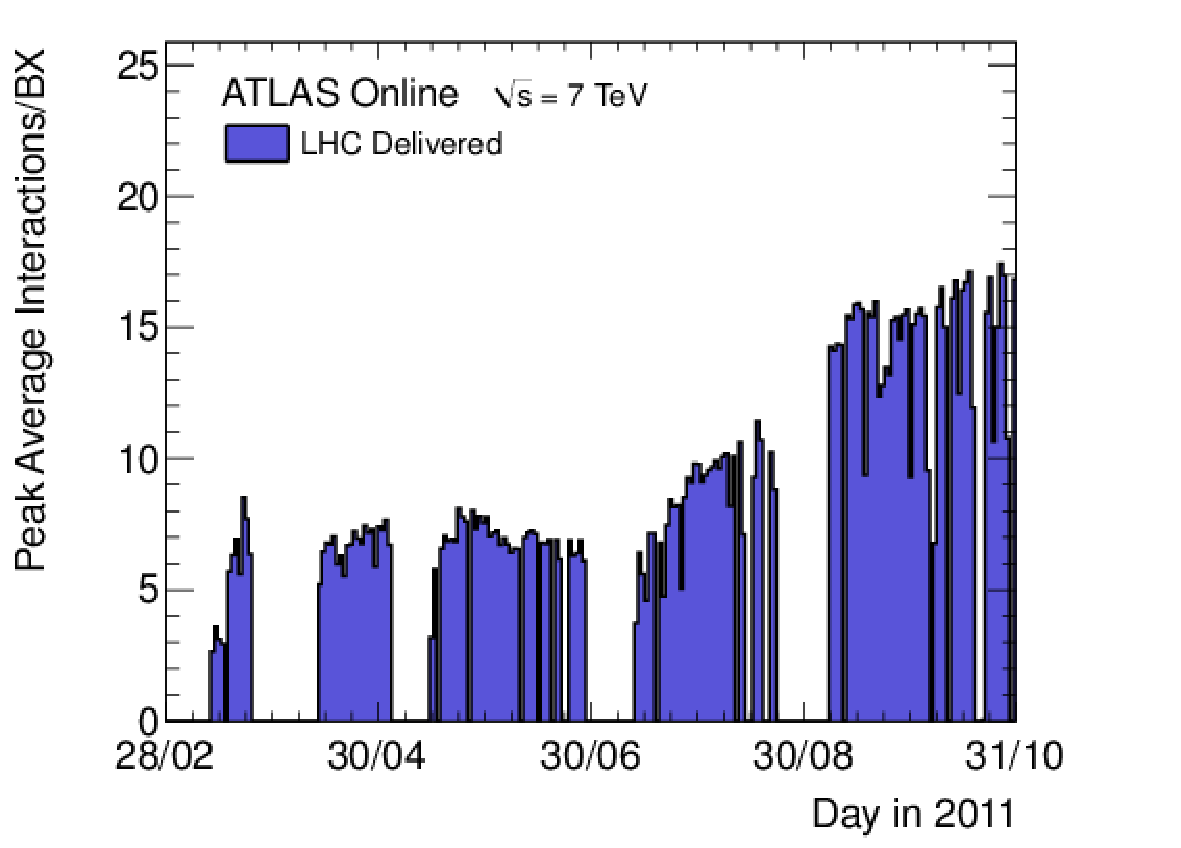
\includegraphics[width=0.7\textwidth]{Fig2/peakAvgMuByDay.pdf}
    \caption{The maximum mean number of events per beam crossing versus day in 2011.}
    \label{fig:peakAvgMu}
  \end{center}
\end{figure}


%------------------------------------------------------------------------
\subsection{Luminosity and pile-up}\label{sec:lumiintro}
%------------------------------------------------------------------------

The rate of events produced by the colliding beams depends on the luminosity of the collisions, which is a measure of the number of events per second per unit cross section, typically measured in units of cm$^2$s$^{-1}$. The number of events of a particular process, then, is given by the product of the integrated luminosity, $\int dt L$, and the cross section of the process, $\sigma_{event}$.  The integrated luminosities are typically quoted in units of inverse picobarns, pb$^{-1}$~=~10$^{-36}$cm$^{2}$. In order to measure processes with very little cross sections a very high luminosity is required. 

The delivered luminosity can be written as~\cite{ATLAS-CONF-2011-116}:

\begin{equation} 
\mbox{ {\it L }} = \frac{n_b f_r n_1 n_2 }{2\pi \Sigma_x \Sigma_y}
\label{eqn:lumi}
\end{equation} 
where $n_b$ is the number of colliding bunch pairs,  $n_1$ and $n_2$ are the bunch populations (protons per bunch) in beam 1 and beam 2 respectively (together forming the bunch charged product), $f_r$ is the machine revolution frequency, and $\Sigma_x$ and $\Sigma_y$ are the width and the height of the proton beams. %characterize the horizontal and vertical profiles of the colliding beams. 

The number of protons per bunch, the number of bunches per beam, and the revolution frequency are all set by the beam operators. The widths of the proton beams are measured in a process known as a Van der Meer ($vdM$) scan~\cite{vanderMeer:296752}. In a $vdM$ scan, the beams are separated by steps of a known distance. The collision rate is measured as a function of this separation, and the width of a gaussian fit to the distributions yields the width of the beams in the direction of the separation.  

The total integrated luminosities provided by the LHC and recorded by ATLAS in 2011 are shown in Figure~\ref{fig:integratedlumi}. These events form the dataset analyzed in this thesis. By means of the beam-separation or $vdM$ scans, as well as other techniques to measure the bunch charged product, the ATLAS Collaboration has determined that the uncertainty on its luminosity measurement is $\delta L = \pm 3.7$\%. For a complete description of the methods used and the systematic erros evaluated see reference~\cite{ATLAS-CONF-2011-116}.

\begin{figure}[htbp]
  \begin{center}
      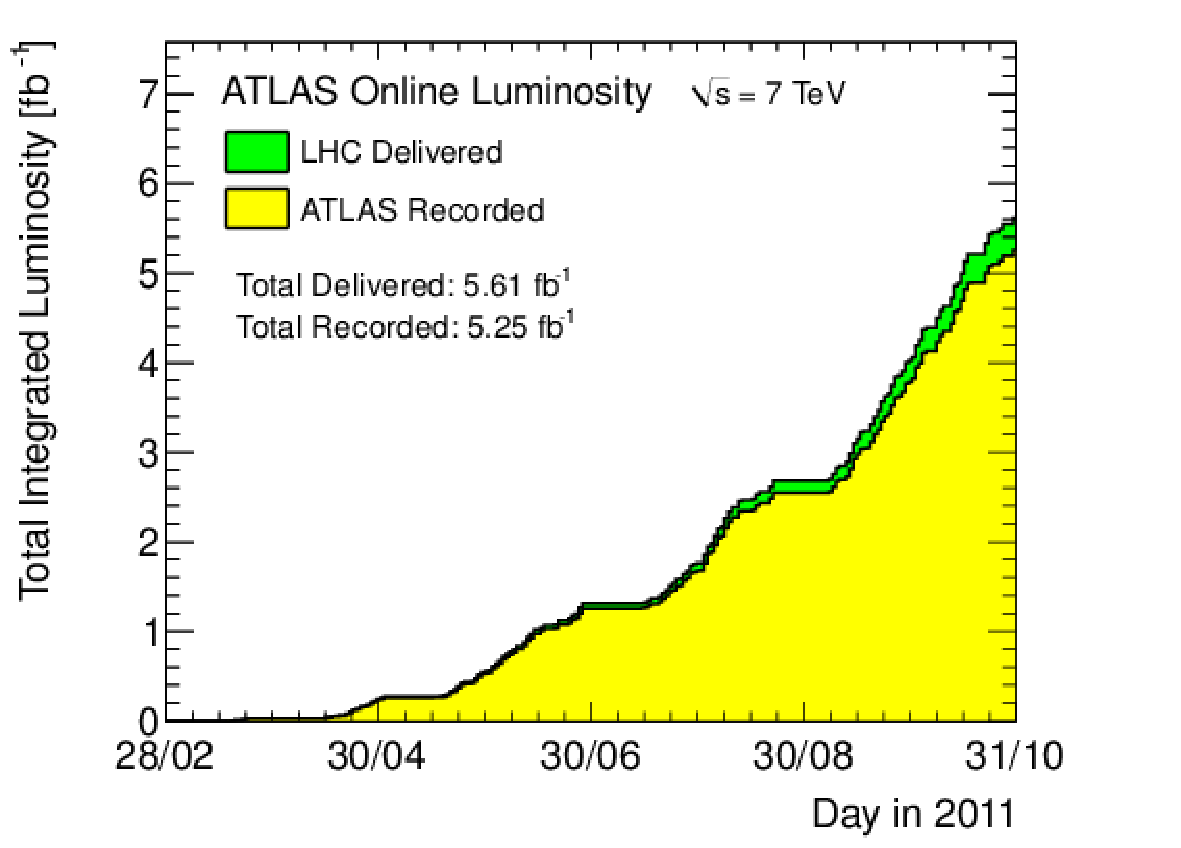
\includegraphics[width=0.7\textwidth]{Fig2/sumLumiByDay.pdf}
    \caption{Total luminosity delivered by the LHC and recorded by ATLAS during the 2011 $\sqrt{s}$ = 7~TeV proton-proton run.}
    \label{fig:integratedlumi}
  \end{center}
\end{figure}


%As anticipated, 
Due to the cross-section for interaction and the large number of protons per bunch, the possibility to observe multiple $pp$ interactions per bunch crossing increases proportionally. This phenomenon, referred to as ``pile-up'', can really occur in two distinct forms. The first form is the presence of multiple $pp$ collisions (different from the interaction of interest) in the same bunch crossing, referred to as ``in-time'' pile-up. The second form of pile-up takes place due to electronic integration times within the detector. Certain detector components are actually sensitive to multiple bunch crossings due to the long electronic signals generated in the response to energy depositions or charge collection. One or more $pp$ collisions in a bunch-crossing different from that which produced the collision of interest can then affect the measurement. This form of pile-up is referred to as ``out-of-time'' pile-up and will become more important as the LHC bunch spacing gets closer to the nominal value, 25~ns.

The fraction of events with pile-up increased significatively since the data taking started. The experimental signature of this fact is obtain via the number of reconstructed primary vertices, or NPV. The effect of the event NPV is an important concern for the measurement of jet properties and will be discussed in the next chapters.


%
%%%%%%%%%%%%%%%%%%%%%%%%%%%%%%%%%%%%%%%%%%%%%%%%%%%%%%%%%%%%%%%%%%%%%%%%%%%%%%%
% ATLAS
%%%%%%%%%%%%%%%%%%%%%%%%%%%%%%%%%%%%%%%%%%%%%%%%%%%%%%%%%%%%%%%%%%%%%%%%%%%%%%%
%
\section{The ATLAS Detector}~\label{sec:ATLASDetector}

%------------------------------------------------------------------------
%\subsection{Detector overview}\label{sec:atlassummary}
%------------------------------------------------------------------------

The ATLAS detector~\cite{ATLAS} is one of the two general purpose particle detectors built for probing $pp$ collisions at the LHC. %As it was described in the previous section, 
Inside the LHC, bunches of up to 10$^{11}$ protons will collide 40 million times per second to provide 14~TeV proton-proton collisions at a nominal luminosity of 10$^{34}$cm$^{-2}$s$^{-1}$; these high interaction rates and energies, as well as the requirements for high precision physics measurements set the standars for the design of the detector. At even 7 TeV center-of-mass energy, the LHC interactions result in high particle multiplicity, requiring fine detector granularity; and, particle production at forward rapidity, requiring large detector angular coverage.

To achieve these performance goals, a design consisting of multiple detector sub-systems with cylindrical symmetry around the incoming beams is used as shown in Fig.~\ref{fig:ATLAS}. Closest to the interaction point the inner tracking detector is placed, providing charged particle reconstruction. The magnet configuration comprises a thin superconducting solenoid surrounding the inner detector cavity, and three large superconducting toroids (one barrel and two end-caps) arranged with an eight-fold azimuthal symmetry around the calorimeters. This fundamental choice has driven the design and size (44~m in length and 25~m in height) of the rest of the detector. Outside the solenoid, a calorimeter system performs electron, photon, tau, and jet energy measurements. %\footnote{}. 
Finally, the calorimeter is surrounded by the muon spectrometer where an array of muon drift chambers perform muon identification and momentum measurements.

The ATLAS detector coordinate system is used to describe the position of particles as they traverse these subdetectors. It is a right-handed coordinate system, with $z$ pointing along the beam direction, positive $x$ pointing toward the center of the LHC ring, and positive y pointing up. The $x-y$ plane is referred to as the transverse plane, and the $z$ direction as the longitudinal
direction. The azimuthal angle $\phi$ is measured as usual around the beam axis, and the polar angle $\theta$ is the angle from the beam axis. The pseudorapidity is defined as $\eta = -\ln (\tan (\frac{\theta}{2}))$, regions of low $\eta$ are referred to as ``central'', and regions of high $\eta$ are referred to as ``forward''. % (in the case of massive objects such as jets, the rapidity y = 1/2ln[(E + pz )/(E − pz )] is used). 
The transverse momentum $\pt$ is defined in the $x-y$ plane unless stated otherwise. The distance $\Delta R$ in the pseudorapidity-azimuthal angle space is defined as $\Delta R = \sqrt{ \Delta \eta^2  + \Delta \phi^2}$ .


\begin{figure}[htbp]
  \begin{center}
      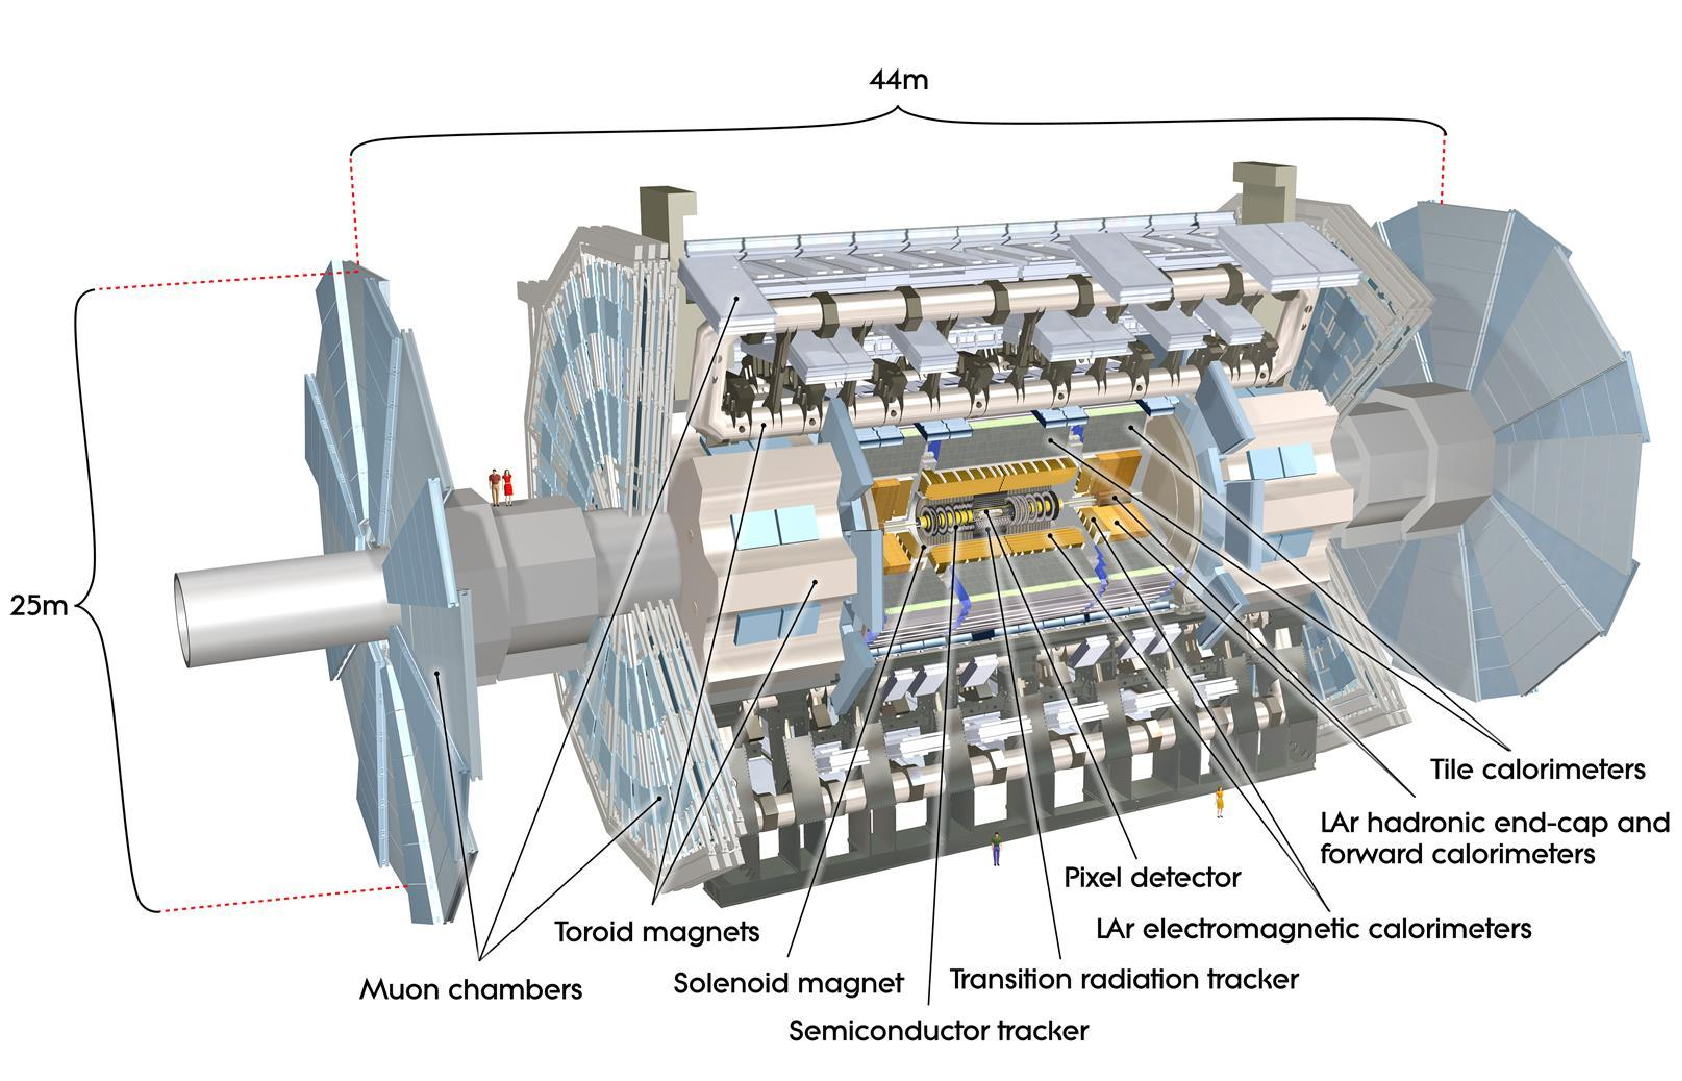
\includegraphics[angle=90,width=1\textwidth]{Fig2/ATLASDetector.pdf}
    \caption{The ATLAS Detector.}
    \label{fig:ATLAS}
  \end{center}
\end{figure}


To meet the extremely high demands that the LHC luminosity places on the speed with which ATLAS must record data, a dedicated trigger and data acquisition (TDAQ) system is used. The interaction rate at the design luminosity is approximately 1~GHz, while the event data recording, based on technology and resource restrictions, is limited to about $\sim$200~Hz. This requires a high rejection of minimum-bias processes while maintaining maximum efficiency for the new physics. The Level-1 (L1) trigger system uses a
subset of the total detector information to make a decision on whether or not to continue processing an event, reducing the data rate to approximately 75~kHz (limited by the bandwidth of the readout system, which is upgradeable to~100 kHz). The subsequent two levels, collectively known as the high-level trigger (HLT), are the Level-2 (L2) trigger and the Event Filter (EF). They provide the reduction to a final data-taking rate of approximately 200 Hz. 



%------------------------------------------------------------------------
\subsection{Inner Tracking System}\label{atlasID}
 %------------------------------------------------------------------------

The inner tracking system or Inner Detector (ID) is composed of three subdetectors: the pixel detector, the semiconductor tracker (SCT) and the transition radiation tracker (TRT). The goal of these three is to provide charged particle trajectory reconstruction and momentum measurements with an overall acceptance in pseudorapidity of $|\eta| < 2.5$ and full $\phi$ coverage. 

The sensors which built this system register signals, referred to as ``hits'', in response to the passage of charged particles. The ID is inmersed in a 2~T magnetic field, generated by the central solenoid. The positions of the registered hits are combined to form tracks, with the radius of curvature  of the tracks (caused by the presence of the magnetic field) providing a measurement of the particle's transverse momentum. 
The track reconstruction efficiency ranges from 78\% at $p^{track}_{T} = 500$~MeV to more than 85\% above 10~GeV, averaged across the full $\eta$ coverage~\cite{chargemultiplicity}. A transverse momentum resolution of $\sigma_{p_T}$/$\pt \aplt 0.05$~\cite{ATLAS-CONF-2010-009} and a transverse impact parameter resolution of $\sim$20~$\mu$m  %for high momentum resolution particles 
for tracks in the central $\eta$ region~\cite{ATLAS-CONF-2010-070} are primarily achieved through the use of high precision subsystems within the ID.

The pixel detector, SCT, and TRT sensors are arranged on concentric cylinders around the beam axis, known as barrel layers, and on disks perpindicular to the beam at either end of the barrel, known as end-caps. A more complete description of these systems is given below. The overall layout of the inner detector is shown in Fig.~\ref{fig:figinner}. 


\begin{figure}[htbp]
  \begin{center}
      \includegraphics[width=0.9\textwidth]{Fig2/InnerDetector.pdf}
    \caption{Layout of the ATLAS Inner Detector.}
    \label{fig:figinner}
  \end{center}
\end{figure}


\subsubsection{The Pixel detector}

The pixel detector consists of three concentric barrel layers. The innermost one, the so called ``$b$-layer'' due to its role in identifying $b$-quarks initiated jets, is located at 5~cm from the interaction region. Three additional disks are located at each end-cap, producing typically three pixel position measurements per charged particle track.  Each layer or disk is instrumented with modules that form the basic unit of data acquisition, each with 47,232 pixels.  All pixel sensors are identical and have a minimum pixel size in $r - \phi \times z$ of 50 $\times$ 400~$\mu m^2$. The intrinsic accuracies in the barrel are 10 $\mu$m in $r - \phi$ and 115 $\mu$m along $z$, or along $r$ in the end-caps. The pixel detector has approximately 80.4 million readout channels, an order of magnitude more readout channels than the rest of ATLAS combined, and it extends to a total length of $z \sim \pm$650~mm and radius of $r \sim$150~mm, providing good reconstruction efficiency for tracks up to $|\eta| <$2.5.

 
\subsubsection{The SCT}


The SCT consists of four barrel layers and nine end-cap layers surrounding the pixel detector, resulting in at least four hits along every charged particle track.  The SCT barrel reaches to $z\sim \pm$750~mm and $r \sim $515~mm, while the end-cap covers out to $z\sim \pm$2720~mm and $r =$560~mm.  There are 15,912 SCT module sensors, each 12.8~cm long and approximately 285~$\mu $m thick. 

In the barrel region, these modules use small-angle (40~mrad) stereo strips to measure both coordinates, with one set of strips in each layer parallel to the beam direction, measuring the $\phi$ coordinate directly . In the end-cap region, the detectors have a set of strips running radially and a set of stereo strips at an angle of 40~mrad. The mean pitch of the strips is 80~$\mu$m. The intrinsic accuracies per module in the barrel are 17~$\mu$m in $r - \phi $ and 580~$\mu$m in $z$ (or $r$ in the end-caps). The total number of readout channels in the SCT is approximately 6.3 million.  A hit is registered only if the pulse height in a channel exceeds a preset threshold ($\sim $ 1~fC). The charged measured in the strip is then recorded into a memory buffer that is only read out and used for tracking if a trigger is received signaling that the event should be considered in more detail.


  
\subsubsection{The TRT}

The TRT surrounds the silicom detectors and is comprised of up to 76 layers of longitudinal straw tubes in the barrel, extending to $z\sim \pm$710~mm and $r \sim$1060~mm, and 160 radial straw planes in each end-cap cylinders, reaching $z\sim \pm$2710~mm and $r \sim$1000~mm.

 The TRT sensors are thin drift tubes consisting of cathode metal straws filled with an ionizing gas mixture of xenon, oxygen, and CO$_2$, with an anode wire running down the center of the straw. The passage of a charged particle through the gas produces positive ions and free electrons, which travel to the cathode and anode, respectively, under the influence of an applied voltage of 1600~V. Comparing the time that the signals are received at the cathode and the anode gives a drift time measurement that can be used to calculate the impact parameter of the particle. This method gives no information on the position along the length of the straw.

To give the best resolution of particle trajectories as they bend in the solenoidal field, the straws lie along the beam direction in the barrel and radially in the end-caps. The straw diameter of 4~mm causes a maximum drift time of approximately 48~ns and an intrinsic accuracy of 130~$\mu$m along the radius of the straw.

In addition to directly detecting charged particles produced by the collision, the TRT also measures the transition radiation induced by the passage of these particles through polypropylene sheets placed between the drift tube straws. Transition radiation refers to the photons emitted by charged particles as they pass from one material into another with a different dielectric constant. These photons yield a much larger signal amplitude than the charged particles, so separate thresholds in the electronics can be used to distinguish the two.

 
 % Este sistema de detecci\'on por tubos provee un gran n\'umero de puntos por traza (t\'ipicamente 36 puntos), lo cual determina un seguimiento cont\'inuo de la misma, con mucho menos material por punto y menor costo (mucho menor comparado con la tecnolog\'ia de p\'ixeles implementada en el subdetector m\'as interno).  La gran cantidad de puntos o impactos por traza es un instrumento poderoso en la b\'usqueda y reconstrucci\'on de trazas en el detector interno.

One of the most important tasks of the inner detector is to provide accurate collision vertex identification, exploiting the excellent position resolution and tracking efficiency. Vertices are reconstructed by matching inner detector tracks with $\pt >$ 150~MeV back to a common origin.% [67].

%------------------------------------------------------------------------
\subsection{The Calorimeter System}\label{sec:atlasCALO}
%------------------------------------------------------------------------

The purpose of the ATLAS calorimeter system is to measure the energy of electrons, photons, taus and jets, within the pseudorapidity region of $|\eta| < $4.9 and with full $\phi$ symmetry and coverage around the beam axis. It also provides fast position and energy measurements to serve as trigger signals for these objects as well as the missing transverse energy. 

The calorimeter detector consist of electromagnetic (EM) calorimeter and hadronic calorimeter components. The EM calorimeter provides fine granularity measurements of electrons and photons.  Each calorimeter is segmented both transverse to the particle direction, to give position information, and along the particle direction, to chart the development of the particle shower.  This permits detailed mapping of EM and  hadronic showers in the calorimeter, allowing for studies of the internal structure of hadronic jets and partially giving rise to the high resolution measurements of their energy.
%%%%%provides detailed information on the transverse and longitudinal shower shapes of hadronic jets.

%It consists of an electromagnetic (EM) calorimeter covering the pseudorapidity region $|\eta| < 3.2$, a hadronic barrel calorimeter covering $|\eta| < 1.7$, hadronic end–cap calorimeters covering $1.5 < |\eta| < 3.2$, and forward calorimeters covering $3.1 < |\eta| < 4.9$. 
The EM and hadronic calorimeters are sampling calorimeters meaning that they utilize alternating layers of absorber material, composed of heavy atoms that interact with energetic particles and cause them to loose energy, and an active material, that produces a signal in response to the deposited  energy.

The calorimeters closest to the beam-line are housed in three cryostats, one barrel and two end-caps. The barrel cryostat contains the electromagnetic barrel calorimeter, and the two end-cap cryostats each contain an electromagnetic end-cap calorimeter (EMEC), a hadronic end-cap calorimeter (HEC), located behind the EMEC, and a forward calorimeter (FCal) to cover the region closest to the beam.  These calorimeters use liquid argon as the active detector medium and need to be mantained at a constant temperature of $\sim$88K.  Liquid argon (LAr) has been chosen for its intrinsic linear behaviour (production of ionization charge as a function of incident charge), its stability of response over time and its intrinsic radiation-hardness. 

An illustration of all these components can be found in Fig.~\ref{fig:figcalo}. Further specifications are given in the next sections.


\begin{figure}[htbp]
  \begin{center}
      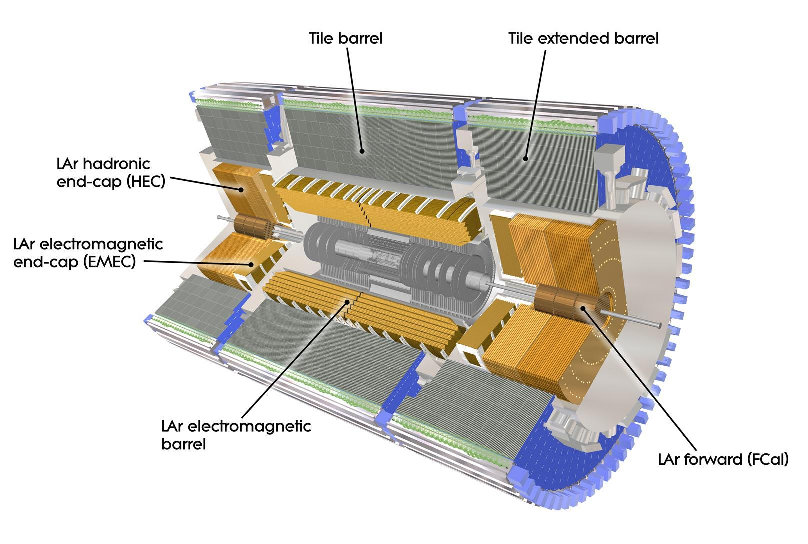
\includegraphics[width=0.9\textwidth]{Fig2/Calorimeters.pdf}
    \caption{Layout of the ATLAS electromagnetic and hadronic calorimeter systems. The total length is $\sim$ 12~m, extending to a maximum radius of 4.25~m.}
    \label{fig:figcalo}
  \end{center}
\end{figure}


\subsubsection{Liquid argon EM calorimeter}
  
The EM calorimeter uses lead as the absorber and liquid Argon as the active material. A photon traversing the absorber will interact with the heavy nucleus via Compton scattering or the photo-electric effect, producing low-energy electrons or; pair production, producing electron/positron pairs. An electron or positron, in turn, can produce bremsstrahlung photons as it is deflected by the nuclei or produce more charged particles via ionization. Thus each incident photon, electron, or positron produces a shower of photons, electrons, and positrons that lose their energy through successive interactions in the absorber. The produced particles ionize the liquid argon, and the charge is collected by electrodes located in the liquid argon gap.  These electrodes consist of three layers of copper sheets, the outer two kept at high-voltage potential and the inner one used to readout the signal.

To provide full coverage in $\phi$ without any cracks, an accordion-shaped absorber and electrode geometry is used, shown in Fig.~\ref{fig:EMacordion}.  This design was chosen to ensure high azimuthal uniformity, a regular liquid argon ionization gap, and a constant sampling fraction within a given detector region. The figure highlights  how this geometry is divided among rectangular cells in $\eta \times \phi$ space, the individual readout elements of varying size,  finely segmented both laterally and longitudinally. Such fine segmentation $– \Delta \eta \times \Delta \phi = 0.025 \times 0.025$ in the second layer of the EM barrel, for example $–$ permits a detailed mapping of the electromagnetic and hadronic showers. 

The position resolution of the EM is driven by the readout geometry (rectangular cells). There are three layers of cells, segmented along the particle's direction of motion.  The $\phi$ segmentation comes from grouping the accordion-shaped electrodes together into a common read out channel. 

In the region $0 <|\eta| < 1.8$ the electromagnetic calorimeters are complemented by a ``presampler'' detector, an instrumented argon layer, which provides a measurement of the energy lost in the solenoid and the outer wall of the barrel cryostat.

The EMEC uses the same accordion geometry as the EMB, whereas the granularity is typically slightly larger than in the barrel.

The signal readout chain for the LAr calorimeter (actually for all calorimeter systems) is divided into a fast analog readout for the trigger system and a slower digital readout used for more redefined trigger decisions and the offline reconstruction. However, regardless of the readout path, the signal is initiated within the active LAr medium. To minimize noise and increase speed the first level of readout is located on the detector (both for LAr and Tile calorimeter, see~\ref{sec:Tile}). The front-end electronics amplify and shape the signal. Shaping electronics induce a bipolar puse shape in the ionization signal. This shape is characterized by having both a positive and a negative component, which renders the integral of the signal exactly equal to zero.

The performance of the shaping electronics is critical for a correct energy calibration of the detector since the energy is primarily determined from the peak height of the pulse. % Figure??
In each calorimeter region, the overall pulse shape and duration are optimized to approximately cancel a constant injection of energy into the detector. The motivation for this approach is to effectively redefine the baseline of the energy measurement. In the high luminosity environment of the LHC, this reduces the sensitivity to the background from multiple $pp$ interactions on average.

To translate these analog signals to digital signals that can be transmitted long distances to the next stage of the readout system, the pulse shape is measured over several 25~ns (nominal) time intervals, known as samples. The challenge of calorimeter calibration is to map these measured signals to the energy deposited in the active detector medium, known as the visible energy. This calibration is established using test-beam measurements of electrons in the EMB~\cite{1748-0221-5-11-P11006,Aharrouche2010400,Aharrouche2007429,Aharrouche2006601} % (REFERENCES) 
and EMEC calorimeters~\cite{Cojocaru2004481,Pinfold2008324}. % (REFERENCES). 


\begin{figure}[htbp]
  \begin{center}
      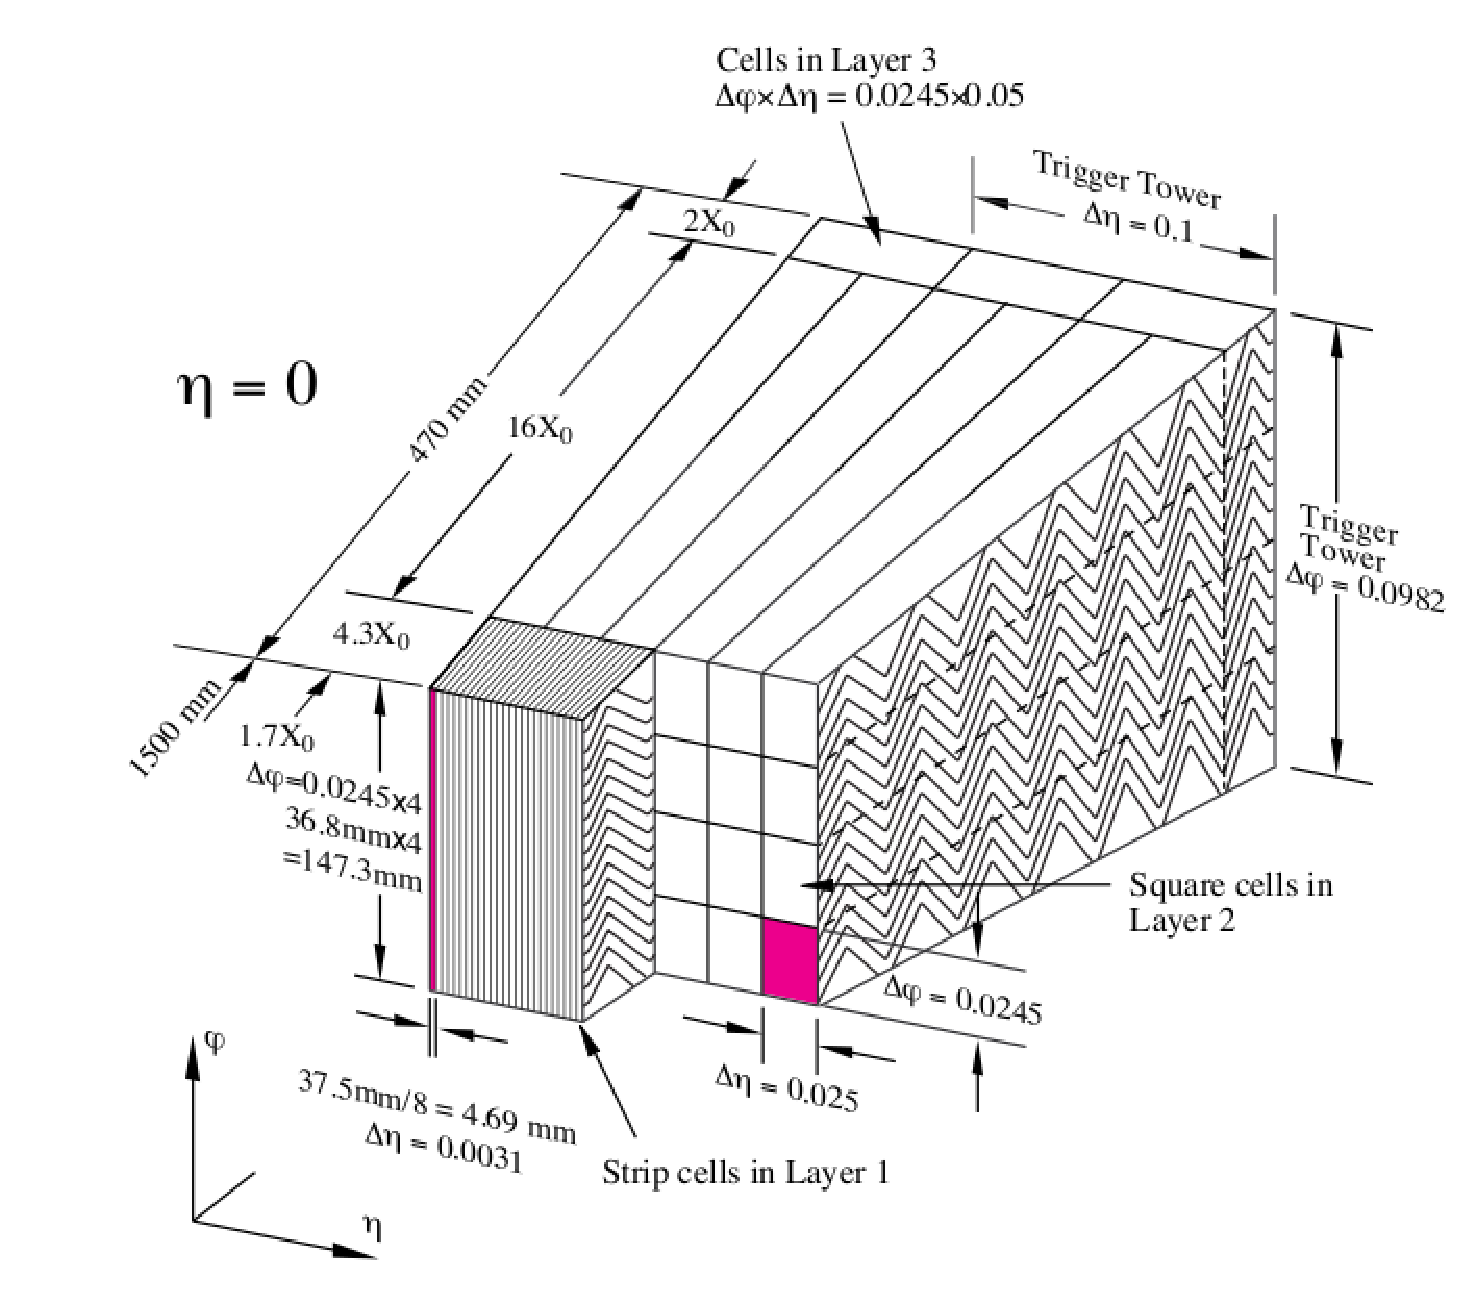
\includegraphics[width=0.9\textwidth]{Fig2/EM_acordionstructure.pdf}
    \caption{Cross section of the LAr barrel calorimeter where the different layers are visible. The granurality in $\eta$ and $\phi$ of the cells of each of the three layers is also shown.}
    \label{fig:EMacordion}
  \end{center}
\end{figure}



\subsubsection{The hadronic calorimeter}\label{sec:Tile}
% TileCal [ ] Tile Calorimeter Technical Design Report, CERN/LHCC 96-42, 15-12-1996;


Outside the EM calorimeter lies the system of hadronic calorimeters. The barrel portion, known as the Tile calorimeter, uses iron absorber slabs interspersed with scintillating tiles. The Tile calorimeter is most notable for its depth of 7.4 radiation lengths ($\lambda$\footnote{To quantify the amount of material needed to capture a particles's energy, the unit of an interaction length, which is the distance over which a high energy charged particle loses $1-\frac{1}{e}\sim 63$\% of its energy , is commonly used.}). The hadronic end-cap and the forward calorimeter, which need to absorb the more energetic particles that are produced at large $|\eta|$, are made of copper and tungsten abosrbers, respectively, with liquid argon as the active material.

The tile calorimeter is composed of 3~mm thick scintillating tiles, arranged to lie parallel  to the incoming particle direction, interleaved with 14~mm thick iron plates. %as shown in Figure!!!!!!!!!!!
It is divided into the barrel calorimeter, covering $|\eta|<1.0$, and two extended barrel calorimeters, covering  $0.8 < |\eta| <1.7$. Each tile is read out by two wavelength-shifting fibers, which convert the scintillator signal to visible light. The readout fibers of several tiles are grouped to a single photomultiplier tube forming cells in $\eta \times \phi$ space. As in the EM calorimeter, these cells are segmented into three layers, the first two of size $\Delta \eta = 0.1$ and  $\Delta \phi = 0.1$ and the last of size   $\Delta \eta = 0.2$ and  $\Delta \phi = 0.1$.  Towers to provide information to the trigger system are formed from 0.1$\times$0.1 grouping of all three layers.

The HEC uses the LAr active readout design due to the higher radiation tolerance required for the forward regions.  Although housed in the same cryostat as the accordion geometry EMEC, the HEC implements a flat-plate design.

The forward calorimeter extends to cover the region $3.1<|\eta|<4.9$. Since it is the only calorimeter that covers this very forward region, it must provide both electromagnetic and hadronic measurements. In addition, the high particle fluxes in this region necessitate a finely granulated design. The FCal is approximately 10 interaction lenghts deep, and consists of three modules in each end-cap: the first, made of copper, is optimised for electromagnetic measurements, while the other two, made of tungsten, measure predominantly the energy of hadronic interactions.

The hadronic calorimeters are calibrated using muons in test-beam experiments % (REFERENCIAS) 
and those muons produced by cosmic-rays in situ. % (see Chapter~\ref{ch:reco}). %(REFERENCIA). 
The invariant mass of the $Z$ boson in $Z \rightarrow ee$ events measured in-situ in the 2010 $pp$ collisions is used to adjust the calibration derived from test-beams and cosmic-muons.





%------------------------------------------------------------------------
\subsection{The Muon System}\label{sec:Muon}
%------------------------------------------------------------------------
 
The muon system gives the ATLAS detector its overall shape and imposing nature, as depicted in Fig.~\ref{fig:MUON1}.
Muons have much smaller cross section to interact in material than electrons and hadrons, for this, they 
do not deposit all their energy in the calorimeters. The muon spectrometer is designed to detect muons within $|\eta|<2.7$. Because many new physics signatures involve high-momentum muons, the system is also required to provide trigger signals based on the particle $\pt$ for  $|\eta|<2.4$.

To provide a momentum measurement, the muons trajectorires are bent in a toroidal magnetic field. This field is provided by one large barrel toroid and two large end-cap toroids, each toroid consisting of eight coils arranged symmetrically around the beam axis.  The toroid system produces a magnetic field that is typically oriented in the $\phi$ direction and that is measured with over 1800 Hall sensors placed throught the magnets. Under the influence of this field, muons are deflected in the $r - z$ plane and the transverse momentum of the muons is given then by the radius of curvature of the tracks. Since the highly-energetic muons bend very little even in this high magnetic field, the muon system is the largest of all the ATLAS sub-detectors, covering a radius from $\sim$4.5~m to $\sim$12.5~m.

Four  primary subsystems comprise the integrated muon spectrometer: monitored drift tubes (MDT), cathode strip chambers (CSC, which are multiwired proportional chambers with cathodes segmented into strips), resistive plate chambers (RPC) and thing gap chambers (TGC). The MDT and CSC subsytems are primarily designed for precision measurements of muon tracks, width the MDT system providing coverage for the more central region ($|\eta|$ < 2.7, with full coverage only in $|\eta| < 2.0$), whereas the CSC is located in the more forward region ($2.0 < |\eta| < 2.7$) due to its ability to cope with higher background rates. The RPC and TGC muon subsystems are desinged to provide fast, robust readout for use in the trigger and data acquisition system.  A detailed description of the subsystems can be found elsewhere~\cite{ATLAS}. 


% Describo todos los sub-systems?
%The MDTs utilize a detector technology very similar to the TRT straws, consisting of anode wires running down the centers of cathode tubes filled with Ar/CO_{2} gas. The passage of a charge particle ionizes the gas atoms, creating free charges that drift to the anode. The time difference between signal at the tube and signal at the wire gives the radial distance of the incident muon track to the wire. The tube diameter of $\sim$30~mm and the operating voltage of 3080~V results in a maximum drift time of 700~ns. The position resolution of each drift tube is 80~$\mu$m along the radius of the tube. 


\begin{figure}[htbp]
  \begin{center}
      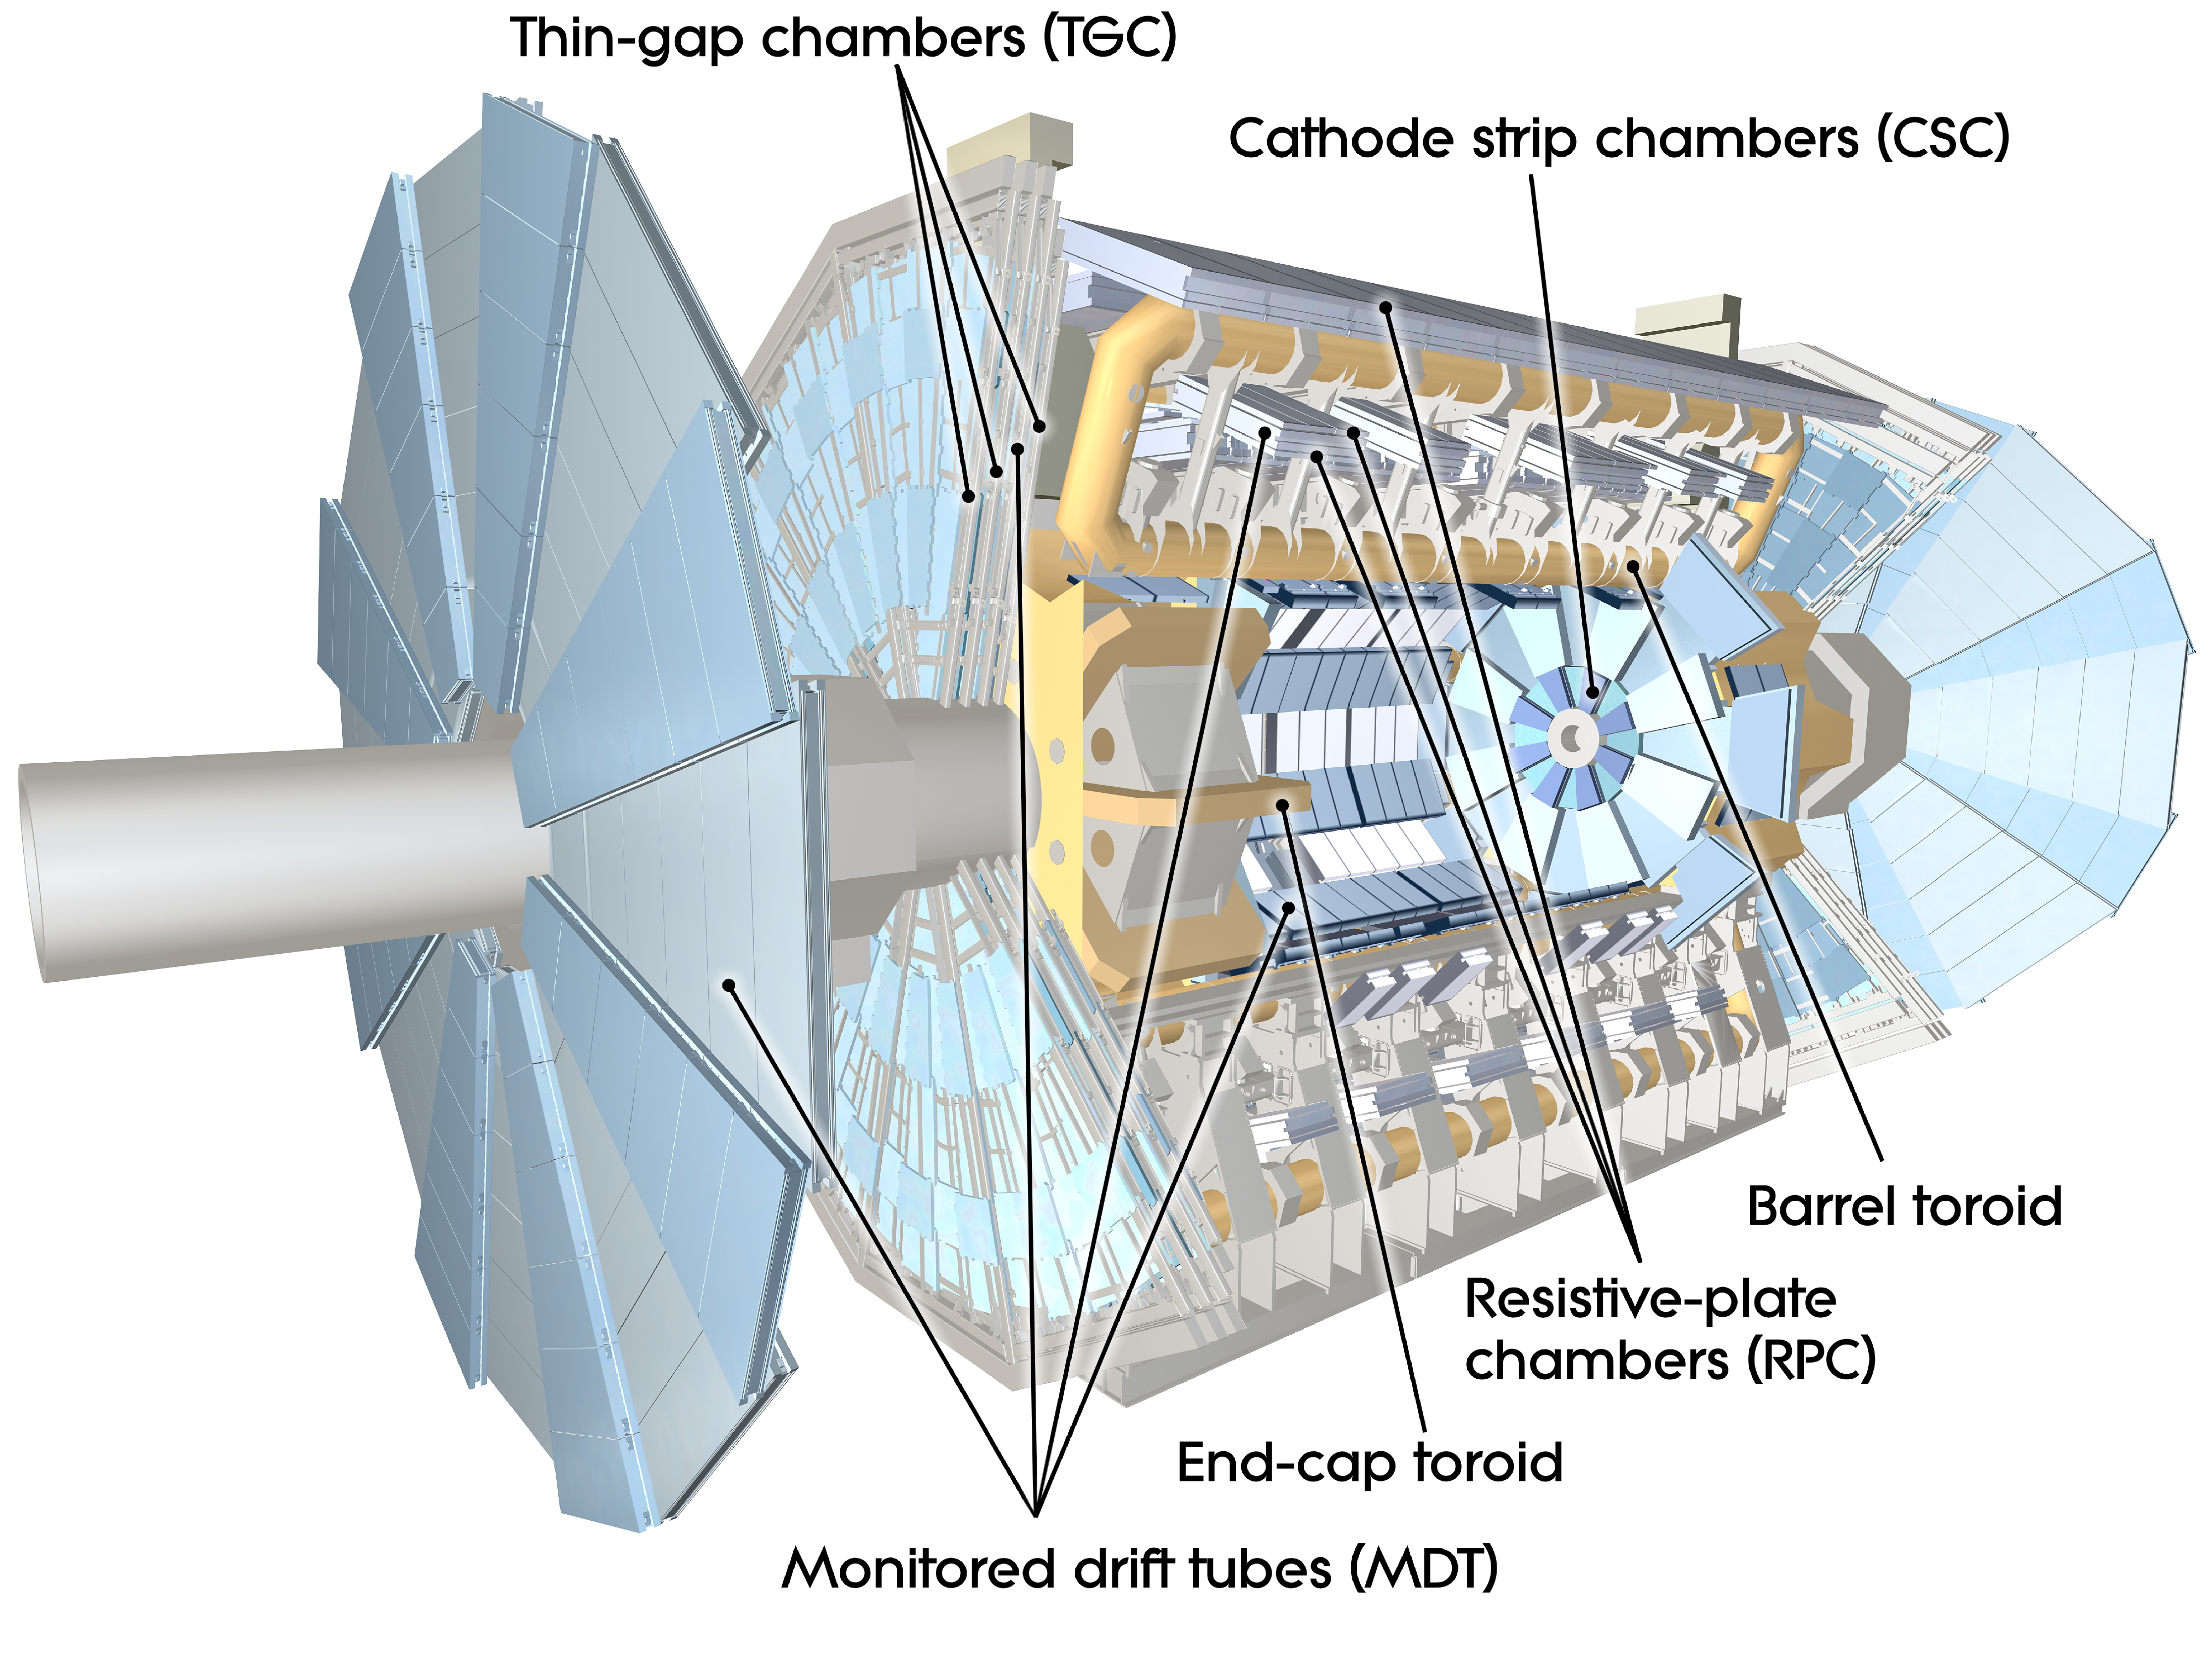
\includegraphics[width=0.8\textwidth]{Fig2/MuonChamber.pdf}
    \caption{The Muon Chamber.}
    \label{fig:MUON1}
  \end{center}
\end{figure}

%------------------------------------------------------------------------
\subsection{Forward Detectors}\label{sec:forward}
%------------------------------------------------------------------------

Three smaller detector systems cover the ATLAS forward region. The main function of the first two systems is to determine the luminosity delivered to ATLAS. At $\pm$17~m from the interaction point lies LUCID (LUminosity measurement using Cerenkov Integrating Detector). The principle of LUCID is to detect inelastic $p-p$ scattering in the forward region, exploiting the fact that the number of particles detectted is proportional to the total, both primary and pile-up, interactions in a bunch-crossing.  LUCID thus provides a relative luminosity measurement, in which the detected number of particles must be translated to the total number of proton-proton interactions via calibration runs.
The second detector is ALFA (Absolute Luminosity For ATLAS). Located at $\pm$240~m, it consists of scintillating fibre trackers located inside Roman pots which are designed to approach as close as 1~mm to the beam. 
The third system is Zero-Degree Calorimeter (ZDC), which place a role in determining the centrality of heavy-collisions.



%------------------------------------------------------------------------
\subsection{Trigger and Data Adquisition System}\label{sec:TDAQ}
%------------------------------------------------------------------------



At design luminoisty, the LHC will deliver approximately 40 million collision events every second. With an average ATLAS event size of $\sim$1.5~MB, this is far more information than can be saved into the finite data storage resources available. The goal of the trigger system is to move interesting physics events to permanent storage, while rejecting the vast majority of other events.

The online selection is done in three stages: the Level 1 (L1), Level 2 (L2) and Event Filter (EF) stages.  Each trigger level refines the decisions made at the previous level and, where necessary, applies additional selection criteria. The data acquisition (DAQ) system  receives and buffers the event data from the detector-specific readout electronics, at the L1 trigger accept rate, over 1600 point-to-point readout links. The L1 trigger uses a limited amount of the total detector information (only from the calorimeter and the muon systems) using only simple hardware based algorithms to make a decision in less than 2.5~$\mu$s, reducing the rate to about 75~kHz. The L2 and EF, collectively referred to as the High Level Trigger (HLT), are based on fast software algorithms running on large farms of commercial processors.  The L2 is the first stage of the ATLAS DAQ system that has access to data from the ID and is capable of doing partial reconstruction of events up to the L1 accept rate. L2 trigger is designed to reduce the rate to approximately 3.5~kHz, with an event processing time of about 40~ms, averaged over all events. The EF reduces the rate to roughtly 200~Hz. Its selections are implemented  using offline analysis procedures within an average event processing time of the order of 4~s.

The L1 trigger is desinged to accept high-$\pt$ muons, electrons, photons, jets, and taus, as well as events with large missing transverse energy or sum energy. It uses signals from the TGCs and RPCs from muon triggers and reduced granularity calorimeter information for electron, photon, jet, tau and total energy triggers. The calorimeter trigger system, which maintains a fast readout independent from the remainder of the calorimeter is known as the Level-1 Calorimeter. % (L1Calo).  
At this level coarse calorimeter information is available in the form of jet elements with $\Delta \eta \times \Delta \phi = 0.2 \times 0.2$ for $|\eta|<3.2$. Jets are reconstructed using a square sliding window algorithm. In addition to coarse jets, the total transverse energy is also measured at the L1. 
The region of the detector corresponding to the location where the L1 thresholds were passed $-$ so called ``region of interest'' (RoI) $-$ are then delivered to the L2 sofware algorithms.

The L2 trigger applies additional energy thresholds and multiplicity requirements using the RoI around triggered L1 objects. For example, the L2 jet trigger retrieves the data from cells surrounding the L1 RoI and constructs jets using a simplified cone jet algorithm. 

The next step and last stage in the trigger chain is the EF, which receives events that have been selected by the L2 triggers and processes the entire event with the full detector granularity instead of only a restricted region. 

The monitoring infrastructure of the HLT supports the real-time accumulation of histograms, and their aggregation across the farm, so that parameters can be extracted from cumulative distributions that contain events from all processor nodes. Beam parameters determined from those live  histograms are transmitted online to the LHC and are also available to fed back into the HLT itself for use by its own trigger algorithms that depend on the precise knowledge of the luminous region. % (such as $b$-jet tagging).



 

 %  En la figura \ref{fig:TDAQ} se muestra un vista simplificada de los principales componentes y funciones.  

%\begin{figure}[!h]
%\begin{center}
%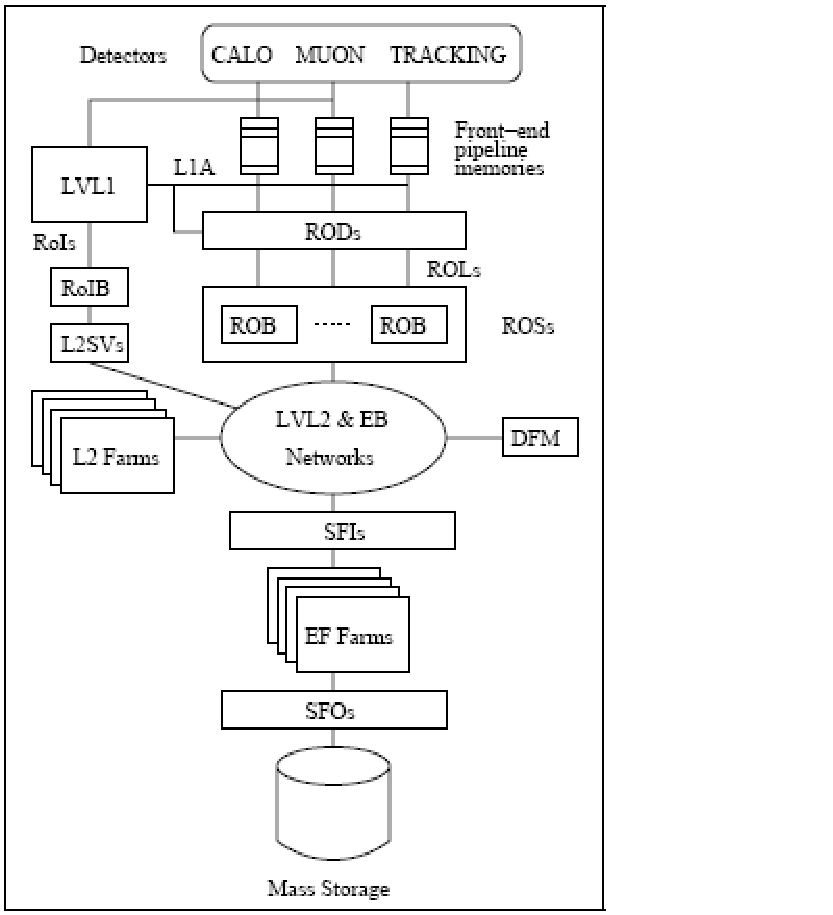
\includegraphics[width=0.5\textwidth]{Fig3/paint_TDAQ.pdf}
%\caption{Principales componentes del sistema de trigger y adquisici\'on de datos de ATLAS. } 
%\label{fig:TDAQ}
%\end{center}
%\end{figure}

  



%------------------------------------------------------------------------
\subsection{ATLAS performance and data quality}\label{sec:DQ}
%------------------------------------------------------------------------

The ATLAS detector has been operational for a number of years collecting large amounts of data. Before the start-up of the LHC, the detector measured 
muons from cosmic rays; which were used to test, understand, and align the detector. In 2010 and 2011 ATLAS recorded over 5.2fb$^{-1}$ of collision data. Fig.~\ref{fig:integratedlumi} presents the luminosity delivered by the LHC in 2011 as well as the recorded luminosity by the detector, showing a good performance of the ATLAS Experiment. 
The fraction of time that each subdetector system was operational during data-taking is shown in Table~\ref{tb:operational}.

The Data Quality (DQ) selection within ATLAS is based on the inspection of a standard set of distributions that lead to a data quality assesment which is encoded in so-called DQ flags. DQ flags are issued for each detector, usually segmented in subdetectors like barrel, end-caps and forward. DQ flags are also issued for trigger slices and for each physics object reconstruction. In this way, the state of the ATLAS detector from hardware to physics object reconstruction is expressed through DQ flags, which are saved per luminosity block. A luminosity block is a time interval of typically two minutes. 

The DQ information is used in analyses through dedicated lists of good runs/luminosity blocks. Good run lists are formed by DQ selection criteria in addition to other criteria, such as run range, magnetic field configuration and beam energy. A complete list of valid physics runs and luminosity blocks is used in each analysis.


\begin{table}[!hbt] %[h]
\renewcommand{\arraystretch}{1.2}
\centering
\begin{tabular}{ | c | c |}
\hline
  ~~~~~~~~~~Detector component~~~~~~~~~~ &~~operational~~ \\ \hline
  Inner Detector         &   \\ 
  ~~Pixel     & $\approx$96.4\%  \\
  ~~SCT       & $\approx$99.2\%  \\
  ~~TRT       & $\approx$97.5\%  \\ \hline 
  Calorimeter               &   \\ 
  ~~EM                      & $\approx$99.8\%  \\
  ~~Tile                    & $\approx$96.2\%  \\
  ~~Hadronic, end-cap       & $\approx$99.6\%  \\ 
  ~~Forward calorimeter     & $\approx$99.8\%  \\ \hline 
  Muon Spectrometer         &   \\ 
  ~~MDT       & $\approx$99.7\%  \\
  ~~CSC       & $\approx$97.7\%  \\
  ~~RPC       & $\approx$97.0\%  \\ 
  ~~TGC       & $\approx$97.9\%  \\ \hline 
\end{tabular}
\caption{The approximate fraction of time that each individual subdetector system was operational during data-taking. }
\label{tb:operational}
\end{table}


%------------------------------------------------------------------------
%\subsection{Simulation of particle interactions in the ATLAS Detector}\label{sec:atlasSim}
%------------------------------------------------------------------------

%HERE????

